\def\layersep{2.5cm}
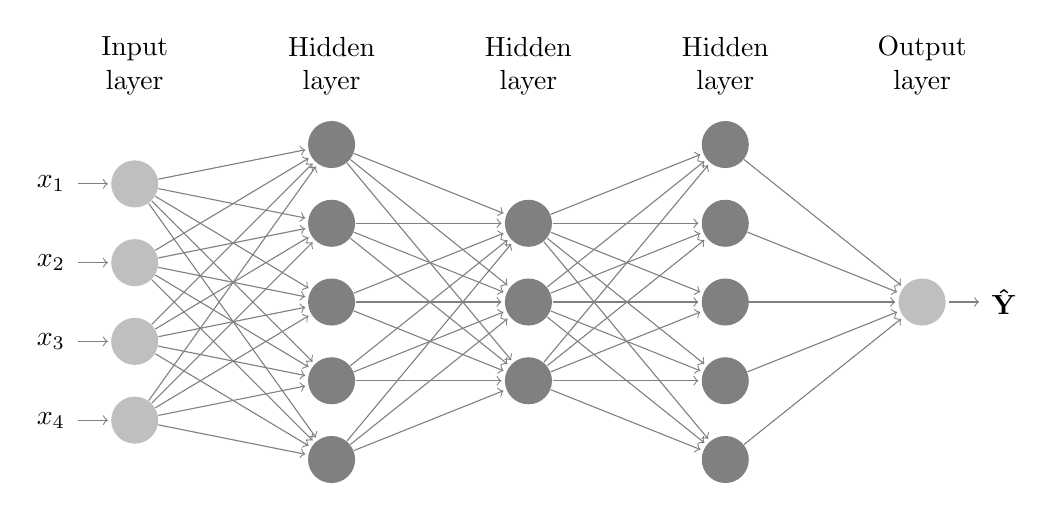
\begin{tikzpicture}[shorten >=1pt,->,draw=black!50, node distance=\layersep]
    \tikzstyle{every pin edge}=[<-,shorten <=1pt]
    \tikzstyle{neuron}=[circle,fill=black!25,minimum size=17pt,inner sep=0pt]
    \tikzstyle{input neuron}=[neuron, fill=gray!50];
    \tikzstyle{output neuron}=[neuron, fill=gray!50];
    \tikzstyle{hidden neuron}=[neuron, fill=black!50];
    \tikzstyle{annot} = [text width=4em, text centered]

    % Draw the input layer nodes
    \foreach \name / \y in {1,...,4}
    % This is the same as writing \foreach \name / \y in {1/1,2/2,3/3,4/4}
        \node[input neuron, pin=left:$x_\y$] (I-\name) at (0,-\y) {};

    % Draw the hidden layer nodes
    \foreach \name / \y in {1,...,5}
        \path[yshift=0.5cm]
            node[hidden neuron] (H-\name) at (\layersep,-\y cm) {};
    % Draw the hidden layer nodes
    \foreach \name / \y in {2,...,4}
        \path[yshift=0.5cm]
            node[hidden neuron] (H2-\name) at (\layersep+2.5cm,-\y cm) {};
    % Draw the hidden layer nodes
    \foreach \name / \y in {1,...,5}
        \path[yshift=0.5cm]
            node[hidden neuron] (H3-\name) at (\layersep+5cm,-\y cm) {};
    % Draw the output layer node
    \node[output neuron,pin={[pin edge={->}]right:$\mathbf{\hat{Y}}$}, right of=H3-3] (O) {};

    % Connect every node in the input layer with every node in the
    % hidden layer.
    \foreach \source in {1,...,4}
        \foreach \dest in {1,...,5}
            \path (I-\source) edge (H-\dest);
            
    \foreach \source in {1,...,5}
        \foreach \dest in {2,...,4}
            \path (H-\source) edge (H2-\dest);
    \foreach \source in {2,...,4}
        \foreach \dest in {1,...,5}
            \path (H2-\source) edge (H3-\dest);

    % Connect every node in the hidden layer with the output layer
    \foreach \source in {1,...,5}
        \path (H3-\source) edge (O);

    % Annotate the layers
    \node[annot,above of=H-1, node distance=1cm] (hl) {Hidden layer};
    \node[annot,above of=H2-2, node distance=2cm] (hl2) {Hidden layer};
    \node[annot,above of=H3-1, node distance=1cm] (hl3) {Hidden layer};
    \node[annot,left of=hl] {Input layer};
    \node[annot,right of=hl3] {Output layer};
\end{tikzpicture}